\section{Design}

\subsection{Component View}

\begin{frame}{\currentname}

\begin{columns}[c]
  \begin{column}{.4\textwidth}
    \begin{small}\textbf{Data Base:} Store all the information about users, zones, queues, drivers position and state, reservations \ldots
        
        \textbf{Account Manager:} Logins and registrations (check all the constraint). Change drivers state.
        
        \textbf{Call Manager:} Get the correct zone from the client position, find an available driver and send a confirmation to the client.
        
        \textbf{Queue Manager:} Provide the first driver in a queue given a zone and manages drivers adding, removing add moving to the end.
        
        \textbf{Reservation Manager:} Checks if a reservation is valid and when a driver accepts it, the reservation is stored in the database.
        
        \textbf{Notification Manager:} Employed for sending notifications to drivers and clients.
        
        \textbf{Position Utilities:} Return a zone from an address, calculate an estimated time for a call or validate a path for a reservation.
        
    \end{small}
  \end{column}
  \begin{column}{.6\textwidth}
    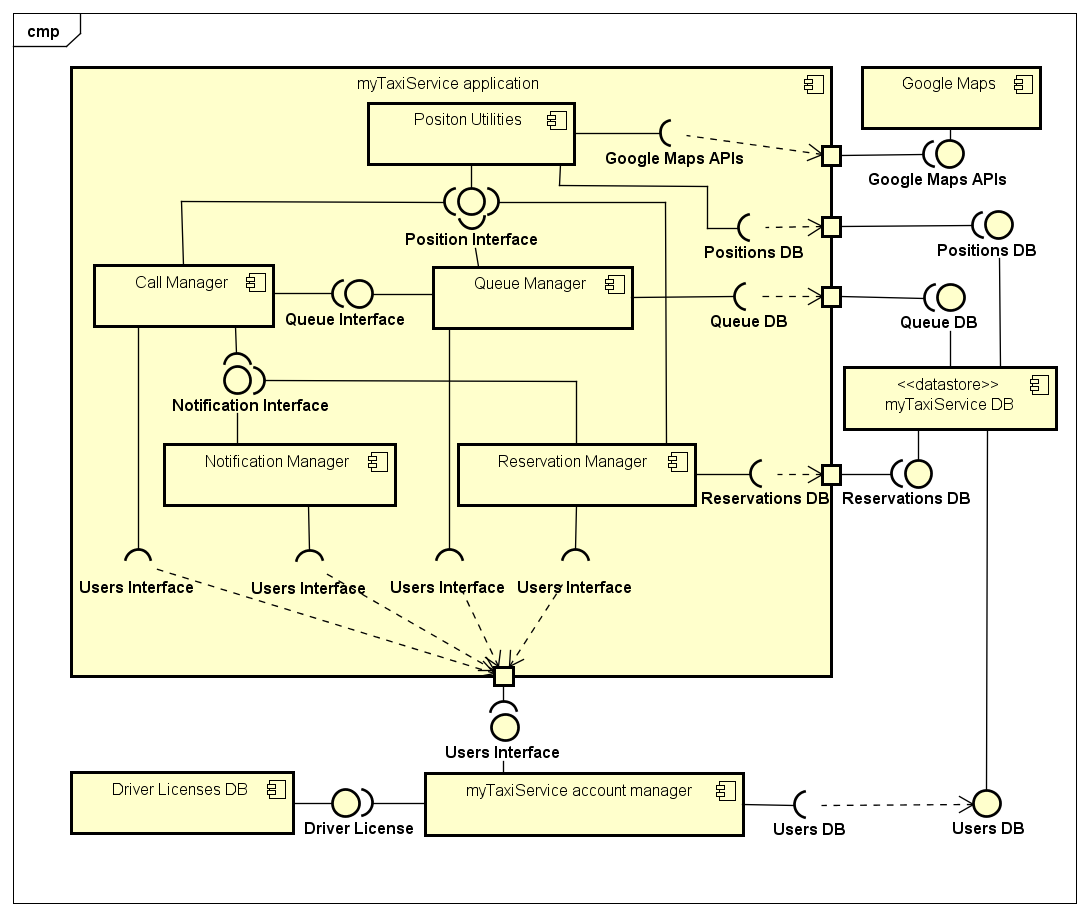
\includegraphics[width=\textwidth]{ComponentDiagram}
	\centering
  \end{column}
\end{columns}

\end{frame}

\subsection{Architectural Style}

\begin{frame}[allowframebreaks]{\currentname}

The system was designed with a \emph{three-tier} architecture: Data, Application Logic and GUI are separated and there are two levels of firewalls in order to keep a high level of security.

\begin{figure}[H]
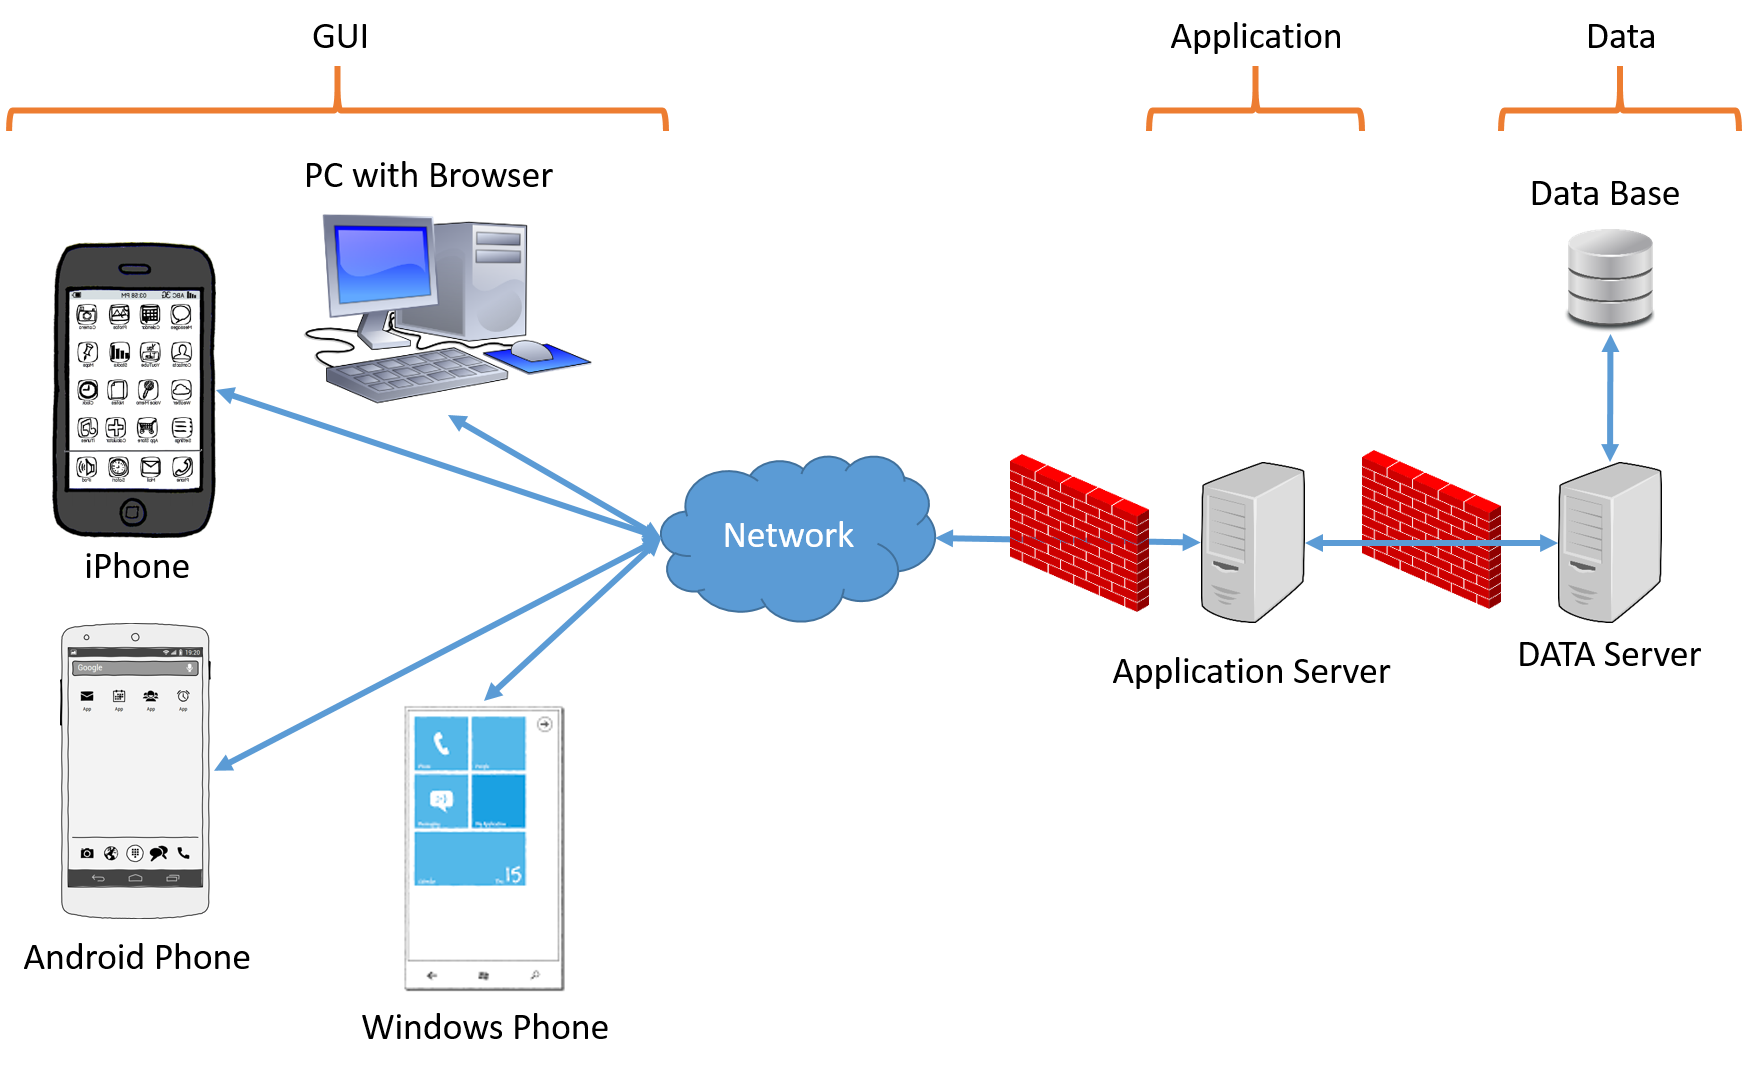
\includegraphics[height=.6\textheight]{Architecture}
\centering
\end{figure}

The \textbf{client server} is used for all the communications which are composed by a request, made by the client, and a response, given by the server.

The \textbf{publisher-subscriber} is needed for the notification service.

\begin{figure}[H]
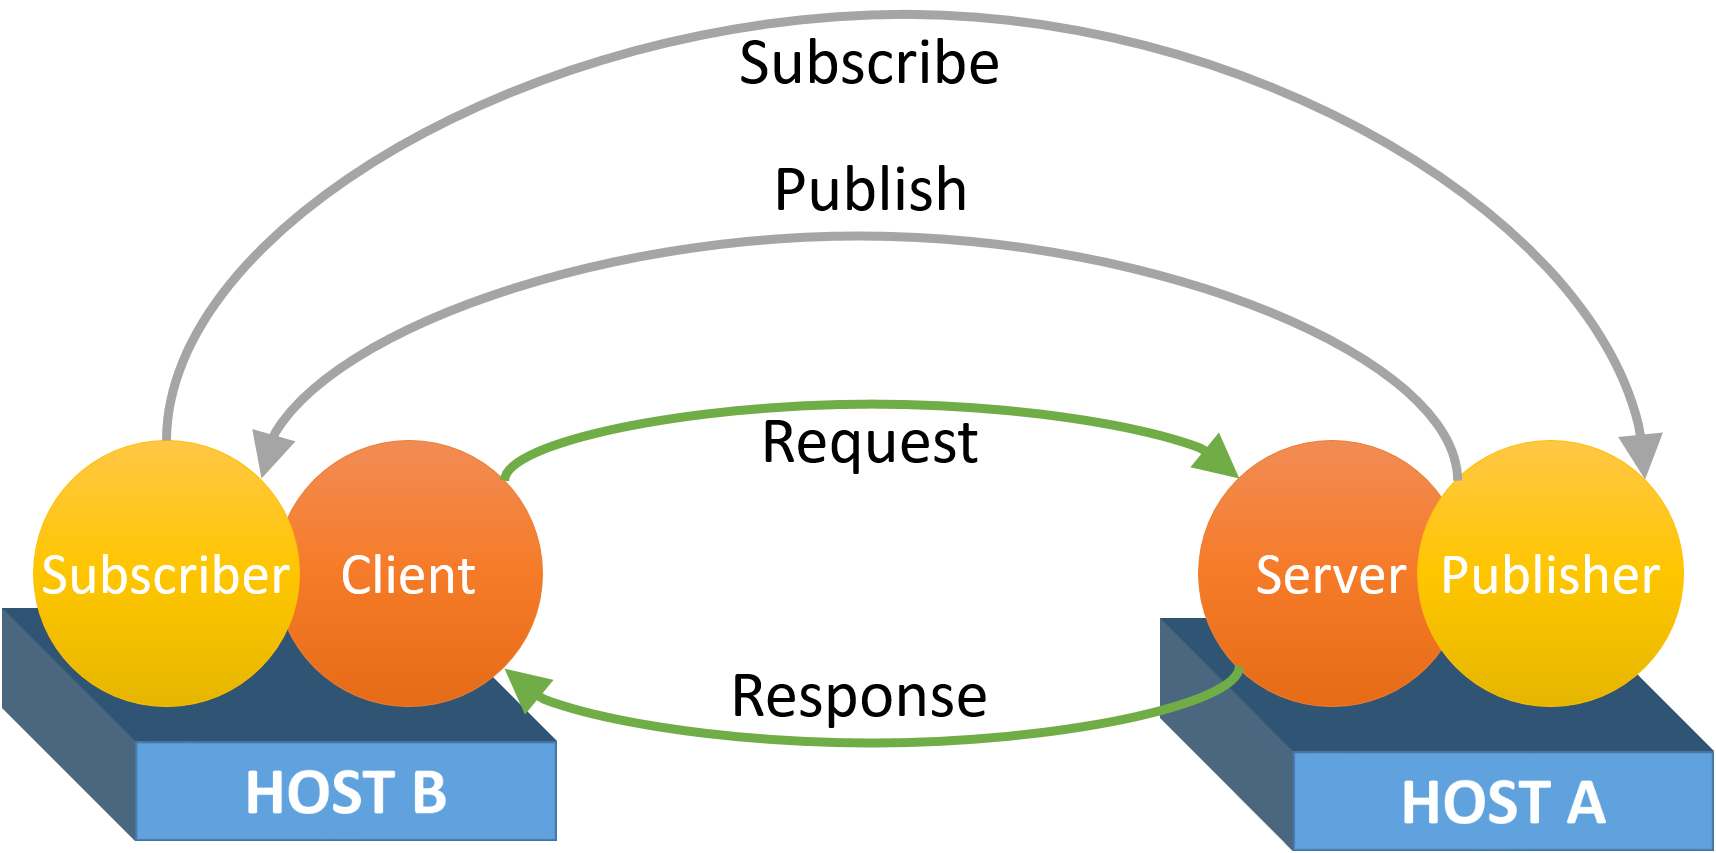
\includegraphics[width=.6\textwidth]{Paradigm}
\centering
\end{figure}

\end{frame}